\SourcePage{GELFAND-P000458}{unlabelled}
\[
H_{\mathbb C}=F^0,\qquad H_{\mathbb Z}\subset H_{\mathbb R}\subset H_{\mathbb C}.
\]
Let there be on $H_{\mathbb C}$ a given bilin. form $\psi$ (nondeg.),
\Unclear{GELFAND-P000458}{first-form}{The sign after “form” reads $\psi$.}
\end{GelfandAdjacentEvidence}
\begin{GelfandAdjacentEvidence}{GELFAND-P000458}{2}

symm. for odd $n$ and skew for even $n$; integral
\Unclear{GELFAND-P000458}{parity-statement}{The manuscript reads “symm. for odd $n$ and skew for even $n$.”}
\end{GelfandAdjacentEvidence}
\begin{GelfandAdjacentEvidence}{GELFAND-P000458}{3}


$\overline D$ — subset in $Z$ of those flags for which
\SourceFigure{GELFAND-P000458}{orthogonality-bracket}{A line encloses the formula from below and at both sides.
\par\smallskip\centering\color{black}
\begingroup\color{black}\GelfandFitDiagram{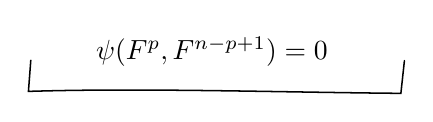
\begin{tikzpicture}[x=1mm,y=1mm,line cap=round]
\node at (25,6.4) {$\psi(F^p,F^{n-p+1})=0$};
\draw[line width=.55pt] (2,5.3)--(1.7,1.35)
  .. controls (16,1.8) and (33,1.25) .. (49,1.1)--(49.45,5.25);
\end{tikzpicture}}\endgroup}
\end{GelfandAdjacentEvidence}
\begin{GelfandAdjacentEvidence}{GELFAND-P000458}{4}


\noindent\rule{\linewidth}{.35pt}

\underline{Add. cond.}\\
\underline{on the flags}\quad $1)\quad F^p\oplus\overline{F^{n-p+1}}\cong H_{\mathbb C}$
\Unclear{GELFAND-P000458}{sum-formula}{The end of the exponent $n-p+1$ is overwritten beside the sign $\cong$.}
\end{GelfandAdjacentEvidence}
\begin{GelfandAdjacentEvidence}{GELFAND-P000458}{5}


$2)$ From it are constr. the grading and the Weil autom. $C$ and then
\[
\psi(x,C\bar y)\quad\text{pos. def. Herm. form on $H_{\mathbb C}$.}
\]
\Unclear{GELFAND-P000458}{weil-link-full}{After $C$ the manuscript reads «и тогда» (“and then”).}
\end{GelfandAdjacentEvidence}
\begin{GelfandAdjacentEvidence}{GELFAND-P000458}{6}


These conditions single out $\underset{\text{(open).}}{D}\subset\overline D$.

$D$ is called the classify. space of Hodge structures.

Depends on the set of dimensions and the form $\psi$.

\underline{Next time}: homogeneity.

grp. of the compl. space $H_{\mathbb C}$, preserv. $\psi$, transit. on $\overline D$

Conn. comp. \(\vphantom{G}_{1}\) grp. of the real space $H_{\mathbb R}$, preserv. $\psi$, transit. on $D$
\Unclear{GELFAND-P000458}{real-prefix}{The left addition provisionally reads «Св. комп.» (“conn. comp.”) with a lowered sign resembling $1$.}
\end{GelfandAdjacentEvidence}
\begin{GelfandAdjacentEvidence}{GELFAND-P000458}{7}


\medskip\noindent\rule{\linewidth}{.35pt}

\underline{Manin’s 2nd lecture}.

\medskip\noindent\rule{\linewidth}{.35pt}

\uuline{D: Kazhdan.}\quad More on Tate’s work.
\Unclear{GELFAND-P000458}{footer-heading}{Two dots sit one above the other after the initial.}



\SourceFigure{GELFAND-P000458}{bottom-mark}{A narrow mark of several strokes crosses the divider. No definite letter or arrow is visible.
\par\smallskip\centering\color{black}
\begingroup\color{black}\GelfandFitDiagram{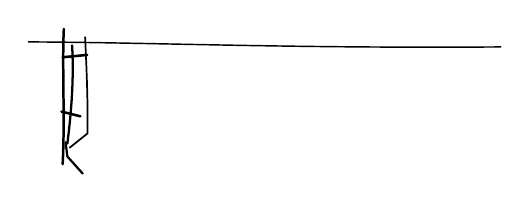
\begin{tikzpicture}[x=.75mm,y=-.75mm,line cap=round,line join=round]
\draw[line width=.52pt] (0,4.6) .. controls (22,4.7) and (43,5.7) .. (80,5.45);
\draw[line width=.9pt] (6,2.4) .. controls (5.7,8.4) and (6.2,18) .. (5.8,25.3);
\draw[line width=.82pt] (7.4,5.2) .. controls (7.8,11.9) and (7,18.6) .. (6.6,21.8);
\draw[line width=.62pt] (9.6,3.8) .. controls (9.9,9.9) and (10.1,15.8) .. (10,20.1)
 -- (7,22.5);
\draw[line width=.92pt] (5.8,7.2)--(9.95,6.8) (5.6,16.4)--(8.8,17.2);
\draw[line width=.8pt] (6.3,21.6)--(6.6,24)--(9.2,26.9);
\end{tikzpicture}}\endgroup}
\end{GelfandAdjacentEvidence}



\Needspace{10\baselineskip}
\section*{Chapter 6}

\Needspace{7\baselineskip}
\begin{GelfandAdjacentEvidence}{GELFAND-P000459}{1}
